\documentclass[twoside,twocolumn]{article}
\usepackage{graphicx}
\usepackage[sc]{mathpazo}
\usepackage[T1]{fontenc}
\linespread{1.05}
\usepackage{microtype}
\usepackage[english]{babel}
\usepackage[hmarginratio=1:1,top=32mm,columnsep=20pt]{geometry}
\usepackage[hang, small,labelfont=bf,up,textfont=it,up]{caption}
\usepackage{booktabs}
\usepackage{lettrine}
\usepackage{enumitem}
\setlist[itemize]{noitemsep}
\usepackage{abstract}
\renewcommand{\abstractnamefont}{\normalfont\bfseries}
\renewcommand{\abstracttextfont}{\normalfont\small\itshape}
\usepackage{titlesec}
\renewcommand\thesection{\Roman{section}}
\renewcommand\thesubsection{\roman{subsection}}
\titleformat{\section}[block]{\large\scshape\centering}{\thesection.}{1em}{}
\titleformat{\subsection}[block]{\large}{\thesubsection.}{1em}{}
\usepackage{fancyhdr}
\pagestyle{fancy}
\fancyhead{}
\fancyfoot{}
\fancyhead[C]{Ethereum 2.0 Client Metrics $\bullet$ \today}
\fancyfoot[RO,LE]{\thepage}
\usepackage{titling}
\usepackage{hyperref}

\setlength{\droptitle}{-4\baselineskip}
\pretitle{\begin{center}\Huge\bfseries}
\posttitle{\end{center}}
\title{Preliminary Ethereum 2.0 Client Metrics for Early Benchmarking}
\author{\textsc{Afri Schoedon, \href{https://github.com/q9f}{@q9f}}}\date{\today}

\begin{document}
\maketitle
\section{Introduction}
\lettrine[nindent=0em,lines=3]{E}thereum 2.0 will be a new blockchain protocol enabling -- amongst others -- horizontal scalability through sharding and transitioning the chain to a proof-of-stake consensus algorithm.\par

None of the features that Ethereum 2.0 will bring are being implemented in established Ethereum 1.x clients such as Geth or Besu. Therefore, it's being worked on a new generation of core clients to power the beacon chain. None of these clients has ever been used in production before.\par

With the launch of the beacon chain supposedly happening in 2020, a first gathering of key metrics of three selected Ethereum 2.0 clients will be conducted, namely Lighthouse, Prysm, and Teku.\par

This article seeks to document the gathered metrics of different clients adhering to scientific methodology. It does not, however, intend to replace a peer-reviewed publication. It's simply a version of the data commented by the author, enriched with emojis. \texttt{;)}\par

The raw data is available on Github\footnote{\href{https://github.com/q9f/eth2-bench-2020-06}{github.com/q9f/eth2-bench-2020-06}} for further analysis.

\section{Clients}
\label{sec:cli}

Three clients are used for comparing key-performance metrics.\par

\begin{figure}[t]
	\centering
	\includegraphics[page=1,width=0.45\textwidth]{../res/plots.pdf}
	\caption{Lighthouse is depicted in orange. All data collected is displayed in this matrix: time running, slot height, blocks per second, database size, memory usage, and peer count.}
	\label{img:lh}
\end{figure}

\begin{figure}[t]
	\centering
	\includegraphics[page=2,width=0.45\textwidth]{../res/plots.pdf}
	\caption{Prysm is depicted in purple. All data collected is displayed in this matrix, same as figure \ref{img:lh}.}
	\label{img:pr}
\end{figure}

\begin{figure}[t]
	\centering
	\includegraphics[page=3,width=0.45\textwidth]{../res/plots.pdf}
	\caption{Teku is depicted in turquoise. All data collected is displayed in this matrix, same as figure \ref{img:lh}.}
	\label{img:tk}
\end{figure}

\textsc{Lighthouse} is an Ethereum 2.0 client developed by Sigma Prime\footnote{\href{https://github.com/sigp/lighthouse}{github.com/sigp/lighthouse}}. It's implemented in the Rust programming language. Data referring to the Lighthouse client is depicted in orange throughout this document (figure \ref{img:lh}).\par

\textsc{Prysm} is a beacon-chain implementation written in Go\footnote{\href{https://github.com/prysmaticlabs/prysm}{github.com/prysmaticlabs/prysm}}. It's being maintained by the Prysmatic Labs team. Data referring to the Prysm client is depicted in purple throughout this document (figure \ref{img:pr}).\par

\textsc{Teku} is an enterprise-grade Ethereum 2.0 client built by the PegaSys Engineering team\footnote{\href{https://github.com/PegaSysEng/teku}{github.com/PegaSysEng/teku}}. It's implemented in Java and data referring to the Teku client is depicted in turquoise throughout this document (figure \ref{img:tk}).\par

Other clients implementing the Ethereum 2.0 protocol exist, namely ChainSafe Systems' \textsc{Lodestar}\footnote{\href{https://github.com/ChainSafe/lodestar}{github.com/ChainSafe/lodestar}}, Status' \textsc{Nimbus}\footnote{\href{https://github.com/status-im/nim-beacon-chain}{github.com/status-im/nim-beacon-chain}}, Nethermind's \textsc{Cortex}\footnote{\href{https://github.com/NethermindEth/cortex}{github.com/NethermindEth/cortex}}, and the Ethereum Foundation's very own \textsc{Trinity}\footnote{\href{https://github.com/ethereum/trinity}{github.com/ethereum/trinity}}. Due to the different progress of implementing the protocol specification and core components, these clients were not considered for comparison, yet.\par

\section{Metadata}
The data is gathered on the Witti testnet\footnote{\href{https://github.com/goerli/witti}{github.com/goerli/witti}}. Witti is the second multi-client testnet launched with the three in section \ref{sec:cli} introduced clients as genesis validators.\par

At the time of collecting the metrics, the Witti testnet is based on \texttt{v0.11.3} of the Ethereum 2.0 beacon-chain specification. It contains approximately 190,000 slots and is run by 989 validators.\par

\subsection{Host Systems}
Three identical host systems have been installed for the sole purpose of the performance inspection. The host systems are virtual private servers with an Arch Linux operating system kernel version \texttt{5.7.2-arch1-1}.\par

The host machines are powered by an AMD EPYC 7281 CPU with 4 virtual cores. The available memory is 12 GiB and the NVMe disk allows for 120GiB capacity.\par

It shall be noted, that these machines are not high-performance machines. This is intentional. The author subjectively tries to create an environment closer to real-world conditions. It is assumed that many users run their beacon-chain nodes \textit{at home}.\par

Furthermore, it shall be emphasized, that this is a preliminary, high-level benchmark. It should be repeated in the future on more appropriate bare-metal machines after stable client-releases are available to eliminate potential performance invariance caused by virtualized systems\footnote{Careful readers will find competition for resources of the three virtualized host systems apparently sharing one physical host in figure \ref{img:sync:sped}.}.\par

\subsection{Client Versions}
All clients were compiled on June 22nd, 2020, from the latest available source-code targeting the version \texttt{v0.11.3} of the Ethereum 2.0 specification.

\begin{itemize}
\item \textbf{Lighthouse}: version \texttt{lighthouse/0.1.2}, compiled from \texttt{master} branch at commit \texttt{710409c2b} with Rust version \texttt{1.44.1} stable through Cargo.
\item \textbf{Prysm}: compiled from \texttt{witti} branch at commit \texttt{172435374} with Go version \texttt{1.14.4} through Bazel.
\item \textbf{Teku}: version \texttt{teku/v0.11.5-dev}, compiled from \texttt{master} branch at commit \texttt{3bd726809} with Java version \texttt{14.0.1} through Gradle.
\end{itemize}

All clients were provided with a sufficient number of bootstrap nodes to ensure good connectivity and eliminate potential networking bottlenecks (compare section \ref{sec:perf} point \ref{sec:perf:p2p}).\par

\begin{figure}[t]
	\centering
	\includegraphics[page=4,width=0.45\textwidth]{../res/plots.pdf}
	\caption{Synchronization progress over time.}
	\label{img:sync:prog}
\end{figure}

\begin{figure}[t]
	\centering
	\includegraphics[page=8,width=0.45\textwidth]{../res/plots.pdf}
	\caption{Synchronization speed over time.}
	\label{img:sync:sped}
\end{figure}

\section{Performance}
\label{sec:perf}
This document does only inspect the performance metrics of beacon-chain node implementations. Other features such as running validator clients, bootstrap nodes, or other relevant tooling is disregarded for simplicity.

\subsection{Synchronization Metrics :)}
Starting this section with an emoji to relax the tension -- synchronization metrics often lead to heated debates on the world wide web.\par

Figure \ref{img:sync:prog} displays the progress of synchronizing the three aforementioned clients. Notably, the Lighthouse client manages to fully synchronize all blocks and verify all signatures in a little less than 1 hour and 49 minutes. Teku completes the same task in 8 hours and 48 minutes, whereas Prysm requires 23 hours and 50 minutes to fully sync and verify the Witti beacon chain.\par

In addition, figure \ref{img:sync:sped} displays the same data but computing the synchronization speed in slots per second by taking the time required to fully catch up with the beacon-chain head. The plotted data points display a moving average over 60 seconds, the plotted line shows a moving average over 10 minutes. Lighthouse appears to be roughly one order of magnitude faster than Teku and Prysm.\par

The data at glance.
\begin{itemize}
\item \textbf{Lighthouse} synchronizes 190,463 slots in 6,539 seconds at an overall average speed of 29.127 slots per second.
\item \textbf{Teku} synchronizes 192,560 slots in 31,688 seconds at an average speed of 6.0767 slots per second.
\item \textbf{Prysm} catches up with 196,943 slots in 85,803 seconds at 2.2953 slots per second.
\end{itemize}

It's important to note that both Teku and Lighthouse do a full verification of all signatures during synchronization \textit{by default} whereas Prysm requires the \texttt{--initial-sync-verify-all-signatures} flag to enable full sync.\par

Assuming a year has 365 days, and the beacon-chain maintains a slot time of 12 seconds, we would see 2,628,000 slots per year. A beacon-chain running under the same conditions as the Witti testnet used for gathering these metrics would require the following synchronization times.

\begin{figure}[t]
	\centering
	\includegraphics[page=5,width=0.45\textwidth]{../res/plots.pdf}
	\caption{Database size over time.}
	\label{img:db}
\end{figure}

\begin{itemize}
\item \textbf{Lighthouse} would require approximately 25 hours to synchronize a year's worth of slots on the Witti testnet.
\item \textbf{Teku} would require around 5 days to synchronize the 2,628,000 slots.
\item \textbf{Prysm} would require circa 13 days for the same task.
\end{itemize}

These numbers are highly hypothetical and should not be taken out of context. Due to finality and weak subjectivity in Ethereum 2.0's proof-of-stake, end-user client synchronization strategies might look very different from what we have experienced in Ethereum 1.x, e.g., by fetching a finalized state and syncing from there.\par

\subsection{Database Metrics}
Figure \ref{img:db} displays the database size in Bytes plotted over time of running the nodes. The patterns are left uncommented for the client developers to analyze.\par

The data at glance.
\begin{itemize}
\item \textbf{Lighthouse} would require 1.89 GiB for 197,068 slots worth of beacon-chain data.
\item \textbf{Teku} would require 3.11 GiB for 197,068 slots.
\item \textbf{Prysm} would require 8.59 GiB for 196,943 slots.
\end{itemize}

Assuming linear growth of the beacon-chain client's databases, we would look at the following yearly growth rates for each client under the conditions comparable to the Witti testnet.

\begin{figure}[t]
	\centering
	\includegraphics[page=6,width=0.45\textwidth]{../res/plots.pdf}
	\caption{Resident memory usage over time.}
	\label{img:mem}
\end{figure}

\begin{itemize}
\item \textbf{Lighthouse} would require 25.8 GiB database space for a year's worth of beacon-chain data.
\item \textbf{Teku} would require 42.6 GiB per year.
\item \textbf{Prysm} would require 117.5 GiB every year under these conditions.
\end{itemize}

However, due to the safe pruning of historic states and advanced database configuration options\footnote{\href{https://lighthouse-book.sigmaprime.io/advanced_database.html}{lighthouse-book.sigmaprime.io/advanced\_database}}, linear growth is not to be expected for end-user clients. Therefore, these data points should be regarded very carefully and only serve as additional context.\par

\subsection{Memory Metrics}
Figure \ref{img:mem} displays resident set size reported by the three clients. Again, the patterns are left uncommented. Notably, the Lighthouse client appears to be most efficient with regard to memory usage, peaking at around 1 GiB in default operation mode. Teku peaks at just below 5 GiB, Prysm at a little less than 8 GiB.\par

\subsection{Networking Metrics}
\label{sec:perf:p2p}
Figure \ref{img:per} displays the peer count of every client during operation. There is not much to be commented on and just serves as a sanity check to rule out networking issues that could impact any of the other metrics.\par

Notably, the drastic drop in peers of the Lighthouse client might be related to a bug that's currently being investigated\footnote{\href{https://github.com/sigp/lighthouse/issues/1272}{github.com/sigp/lighthouse/issues/1272}}.\par

\begin{figure}[t]
	\centering
	\includegraphics[page=7,width=0.45\textwidth]{../res/plots.pdf}
	\caption{Client's peer count over time.}
	\label{img:per}
\end{figure}

\section{Apples and Oranges}
Now, to round this up, an Ethereum 1.x protocol provider will be added to the mix.\par

\begin{figure}[t]
	\centering
	\includegraphics[page=9,width=0.45\textwidth]{../res/plots.pdf}
	\caption{Adding an Ethereum 1.x client to the plot.}
	\label{img:orange}
\end{figure}

Figure \ref{img:orange} adds some context to the synchronization speed depicted in figure \ref{img:sync:sped}. In addition to the data points of Lighthouse, Teku, and Prysm, an \textsc{OpenEthereum}\footnote{\href{https://github.com/openethereum/openethereum}{github.com/openethereum/openethereum}} node is added in black. OpenEthereum is an Ethereum 1.x client implementation maintained by Gnosis.\par

The client was tasked to synchronize and fully verify the first 302,967 blocks on the Goerli testnet\footnote{\href{https://github.com/goerli/testnet}{github.com/goerli/testnet}}. It completed in 295 seconds with an overall average synchronization speed of 1,207 blocks per second making it two orders of magnitude faster than Lighthouse, or even three orders of magnitude faster compared to Teku and Prysm.\par

Furthermore, it managed to synchronize the entire active blockchain of the testnet with 2,924,236 blocks in 4 hours and 15 minutes at an overall average speed of 191.3 blocks per second.\par

\section{Conclusion}
Even though it's early to make any substantial conclusions and the clients are still undergoing very active development, two things cannot be ignored when looking at the data.

First of all, it's difficult to compare Ethereum 1.x clients with Ethereum 2.0 clients due to the entirely different architecture and cryptography they require. However, from a practical perspective, these numbers \textit{do} matter for some -- if not many -- users out there. While being fully aware of the ongoing active development in the Ethereum 2.0 client landscape, we should be encouraged to double down research on increasing these numbers by \textit{orders of magnitude} rather than \textit{some percentage}.\par

Being able to verify a block in 10 milliseconds or less (hypothetical number) is not only faster and more convenient for users but also improves the node's stability and the robustness of the network against denial-of-service attacks.\par

Secondly, a huge shoutout to the Sigma Prime team positioning their Lighthouse client on top in every metric collected. It shall be noted that Ethereum 2.0 is not a race or competition but rather a massive collaborative effort to design and implement a new blockchain protocol. While this is not about calling out a winner, we should be encouraged to learn from the Sigma Prime team's design decisions and the Lighthouse architecture to potentially improve other Ethereum 2.0 node implementations.\par

\begin{figure}[t]
	\centering
	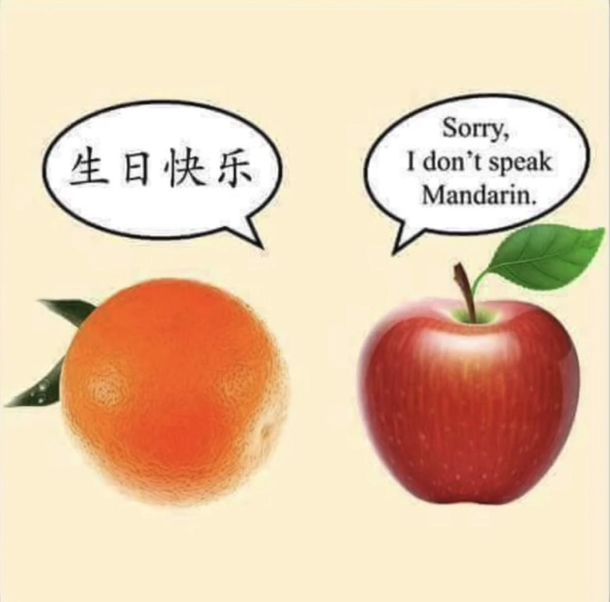
\includegraphics[width=0.45\textwidth]{../res/vegies.png}
	\caption{Apples and Oranges.}
	\label{img:meme}
\end{figure}

\vspace{\fill}

\section*{Note}
The author is not affiliated with any of the teams implementing an Ethereum 2.0 client. The author is independently funded through the Ethereum Foundation's Ecosystem Support Program\footnote{\href{https://esp.ethereum.foundation}{esp.ethereum.foundation}} and the Goerli Testnet Initiative\footnote{\href{https://goerli.net}{goerli.net}}.\par

The author is not speaking on behalf of any organization.\par

Last but not least, the author would like to thank Ronin Kaizen and Franzi Heintel for checking this document for it's integrity and Danny Ryan for giving this data a quick review as well as enough context to rule out common pitfalls analyzing Ethereum 2.0 specification implementations.\par

Thank you.\par

\texttt{:)}
\end{document}
